\chapter{Montaje filawinder}
\label{ane:filawinder}
Para poder almacenar el filamento que vamos extruyendo mediante el Filastruder hemos escogido un kit DIY, llamado Filawinder\cite{filawinder}. 

    \begin{figure}[H]
            \centering
            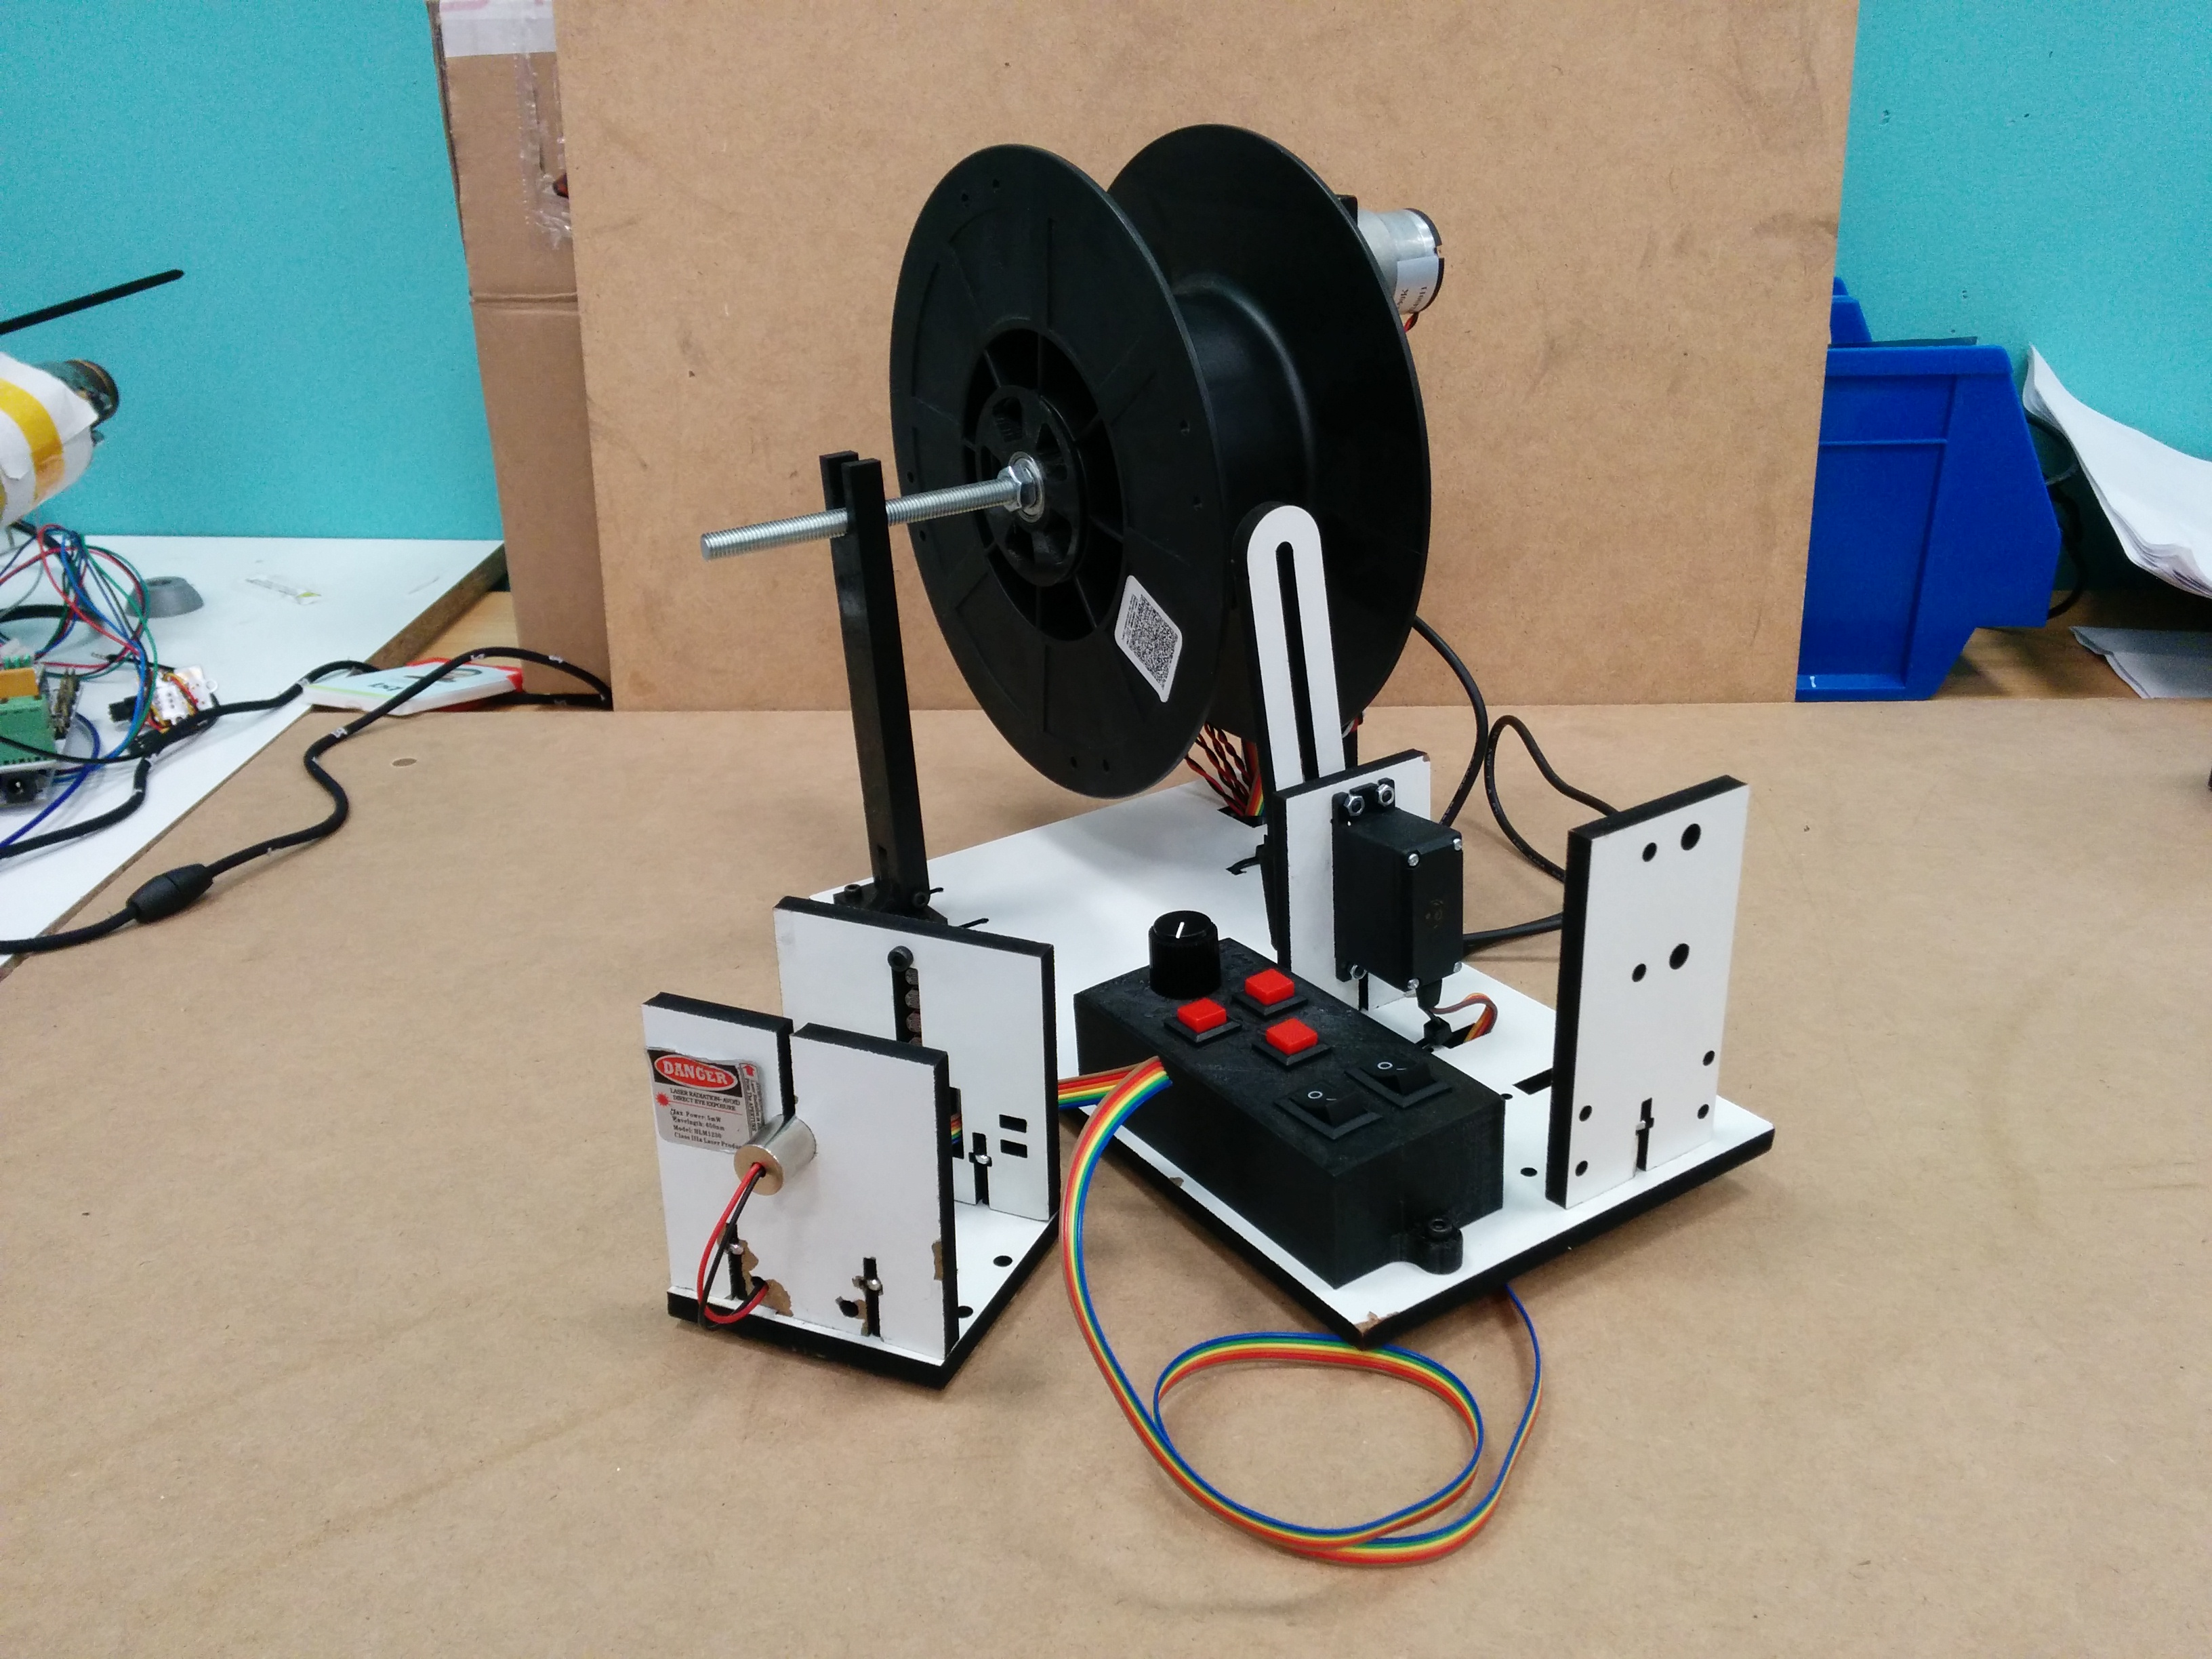
\includegraphics[width=0.4\textwidth]{images/filawinder/IMG_20150313_103643.jpg}
            \caption{Montaje de Filawinder.}
            \label{fig:winder_winder}
    \end{figure}

Filawinder es un kit DIY que se ofrece como expansión a la extrusora  filaextruder. Hemos elegido este en concreto debido a su similitud con una bobinadora de filamento real haciendo así, que la maqueta que vamos a montar sea lo más cercana a la realidad. Otra ventaja es su facilidad de montaje y la amplia documentación disponible en internet.\\

Filawinder es un sistema de almacenamiento de bobinado automatizado. Consiste en un motor en el que va anclado la bobina para almacenar el filamento. La velocidad de giro del motor, está controlada por unos sensores de posición que detectan la tensión del filamento, y en función de ello la velocidad del motor es regulada. Estos sensores resistivos de luz (LDR), funcionan mediante la proyección de la sombra del filamento en ellos para que su resistencia varíe. El filamento, al pasar entre medias del haz y los LDR, irá proyectando la sombra y podremos detectar la tensión del filamento. Logrando así mejorar el almacenamiento del filamento producido.

    \begin{figure}[H]
            \centering
            \includegraphics[width=0.4\textwidth]{images/filawinder/Sensor-filamento.jpg}
            \caption{Sensor de filamento.}
            \label{fig:winder_sensor}
    \end{figure}

También dispone de una guía automática que va moviendo el filamento a lo largo de la bobina, para evitar nudos en su bobinado. Esta guía va teniendo en cuenta el número de vueltas que va realizando la bobina, para ir desplazando el filamento a lo largo del eje transversal de la bobina.\\

Filawinder se distribuye en formato DIY por lo que se venden las piezas sueltas y es necesario que el usuario final realice el montaje. (Ver imagen \ref{fig:winder_material})
    \begin{figure}[H]
            \centering
            \includegraphics[width=0.5\textwidth]{images/filawinder/materiales-filawinder.png}
            \caption{Materiales de filawinder.}
            \label{fig:winder_material}
    \end{figure}

Además de las piezas que se nos suministra, también será necesario tener acceso a una impresora 3D para imprimir unas piezas necesarias para completar el montaje.

    \begin{figure}[H]
            \centering
            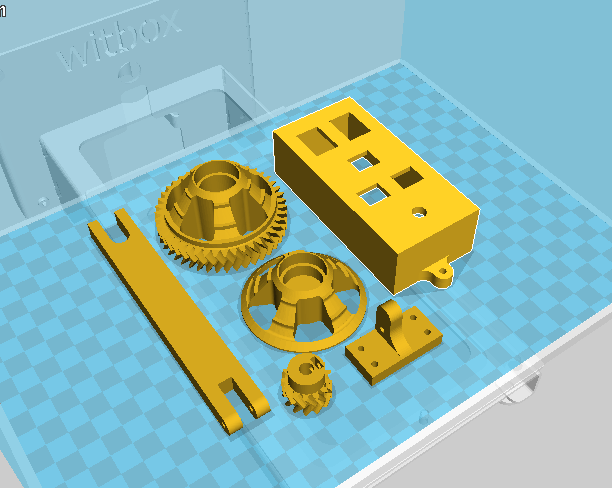
\includegraphics[width=0.5\textwidth]{images/filawinder/piezas-impresas.png}
            \caption{Piezas impresas para filawinder.}
            \label{fig:winder_piezas}
    \end{figure}

 Una vez que ya tenemos todas las piezas disponibles, podremos empezar con el montaje.\\

Alojamos el motor en la pieza destinada a ello. Con ayuda de dos tornillos M3X10 sujetamos el motor a la pieza para evitar que se mueva, pero no hacemos mucha fuerza, ya que la posición final se realizará más adelante.

    \begin{figure}[H]
            \centering
            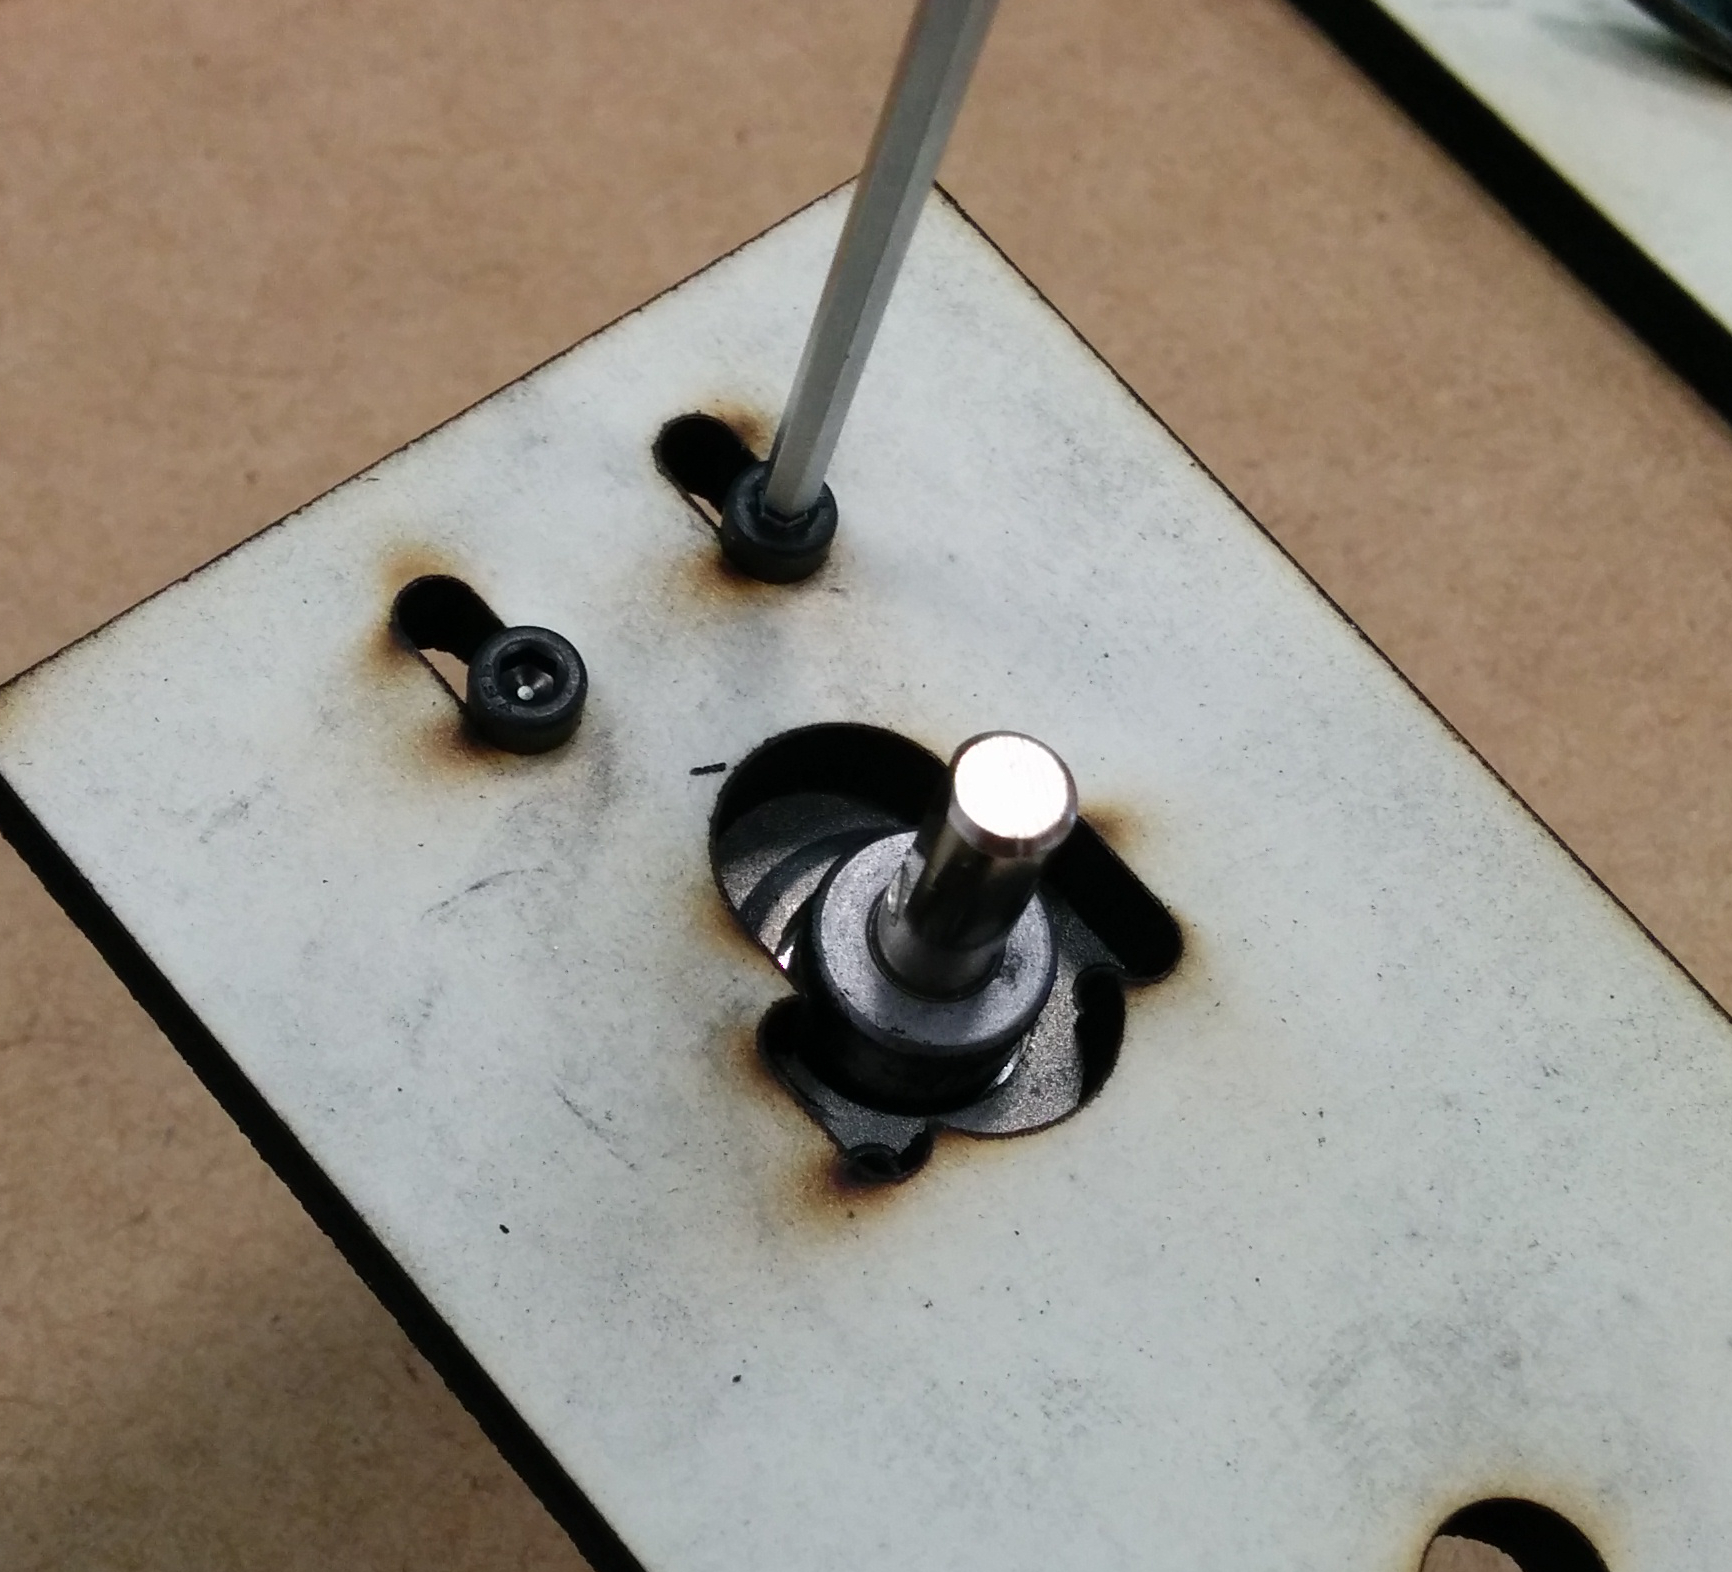
\includegraphics[width=0.5\textwidth]{images/filawinder/montaje1.png}
            \caption{Introducimos el motor en el hueco.}
            \label{fig:winder_piezas1}
    \end{figure}

    Introducimos una tuerca en el alojamiento del engranaje pequeño como se ve en la imagen \ref{fig:winder_engranaje}, para poder apretar el engranaje al vástago del motor con el tornillo de M3x10 (Ver imagen \ref{fig:winder_apriet})
    \begin{figure}[H]
          \centering
        \begin{subfigure}[b]{0.35\textwidth}
                \centering
                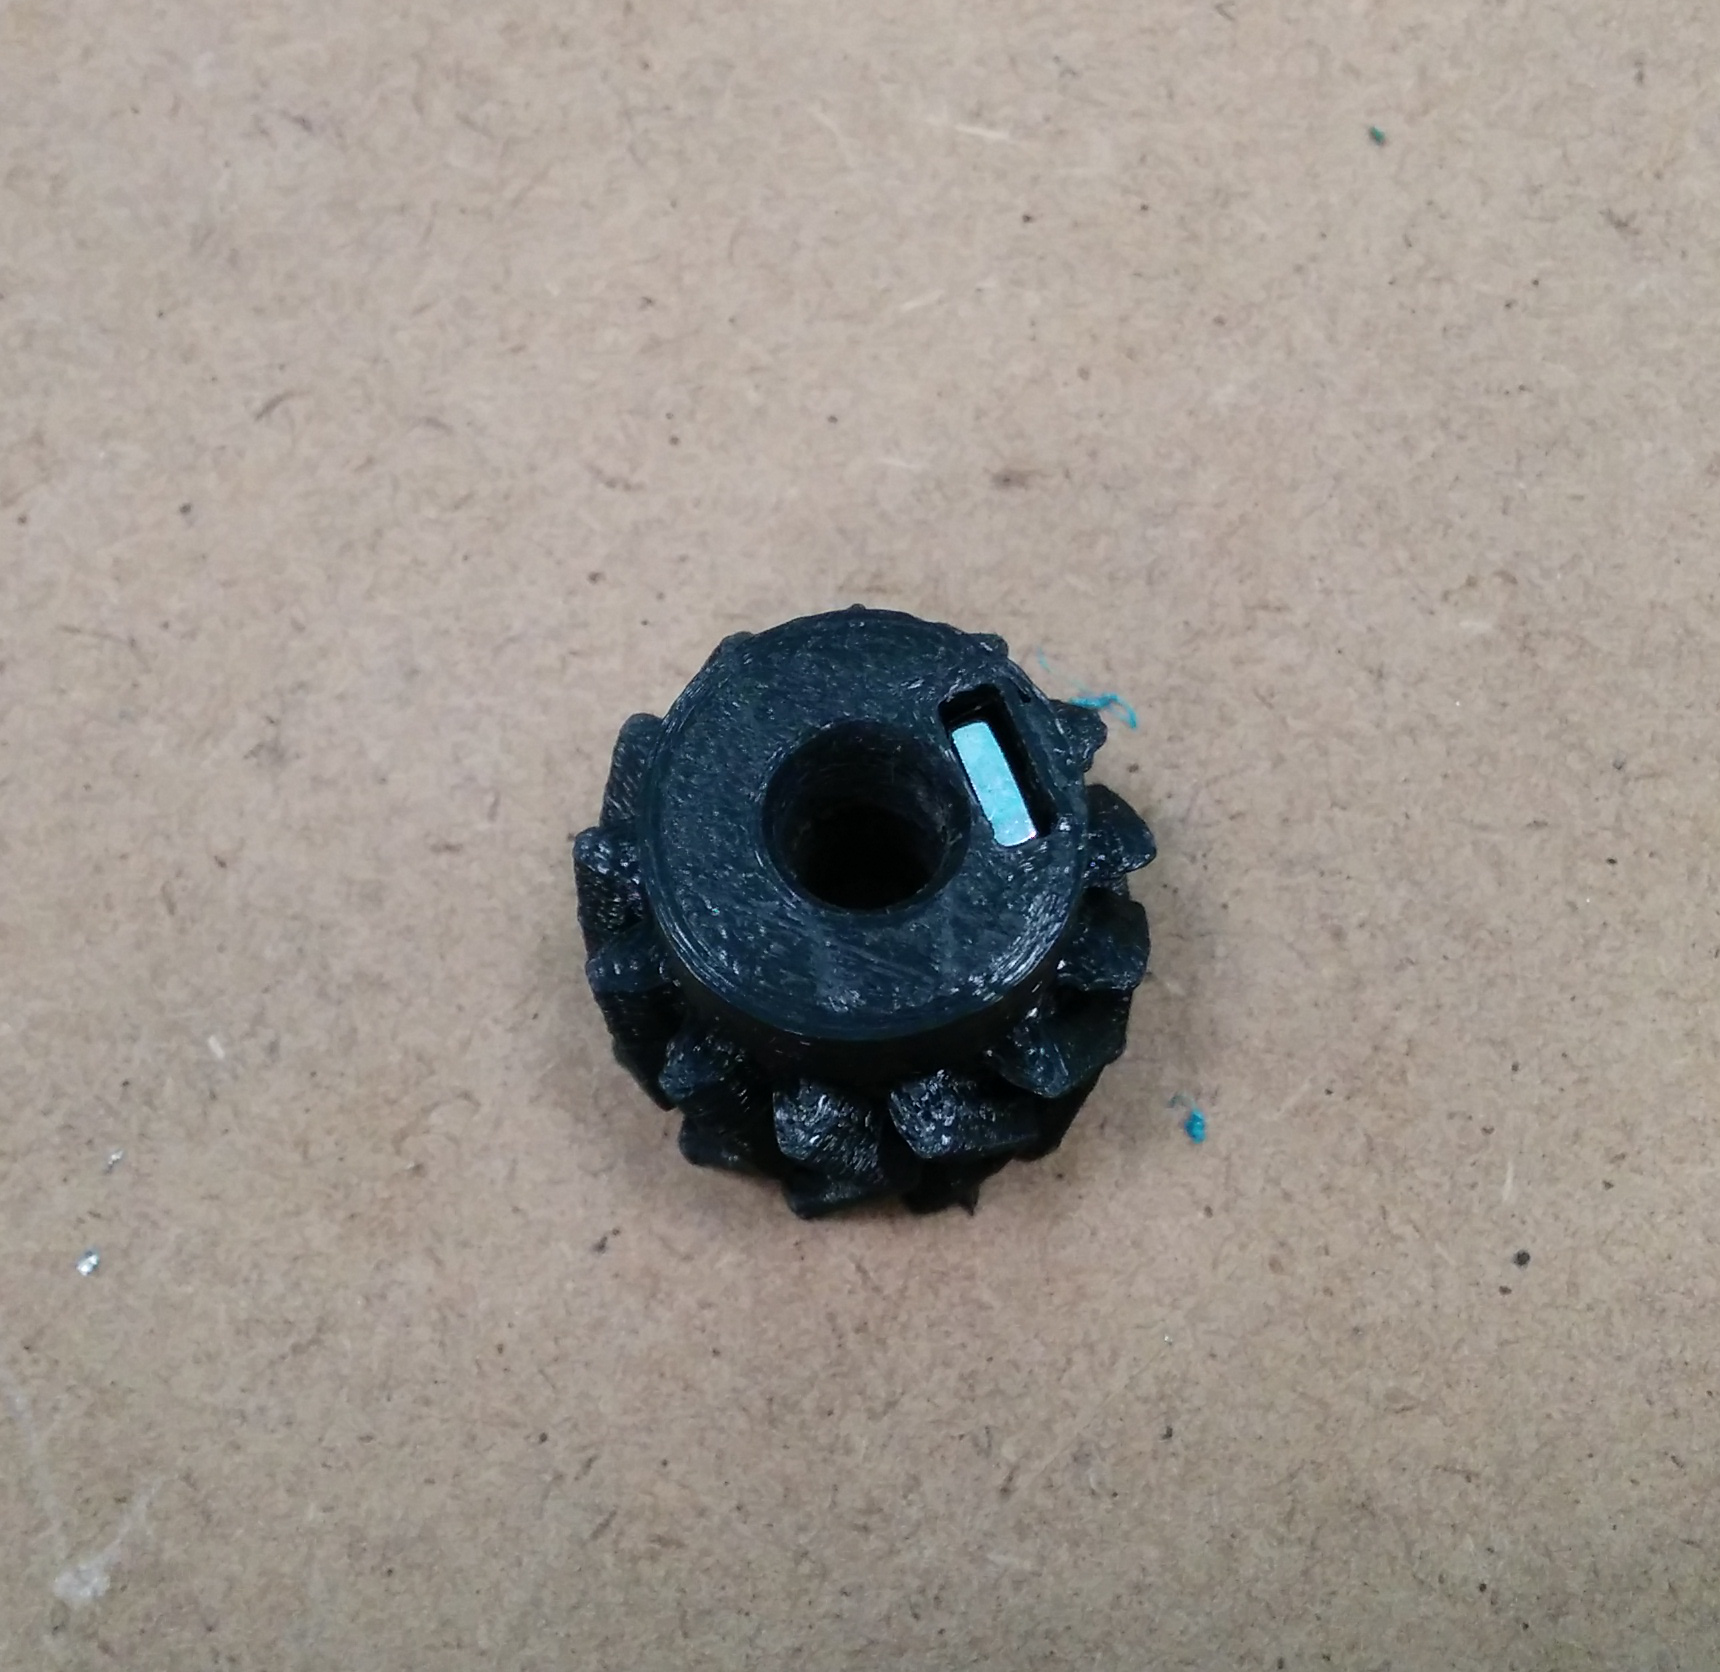
\includegraphics[width=\textwidth]{images/filawinder/montaje2.png}
                \caption{Tuerca en alojamiento de engranaje}
                \label{fig:winder_engranaje}
        \end{subfigure}
        ~
        \begin{subfigure}[b]{0.35\textwidth}
                \centering
                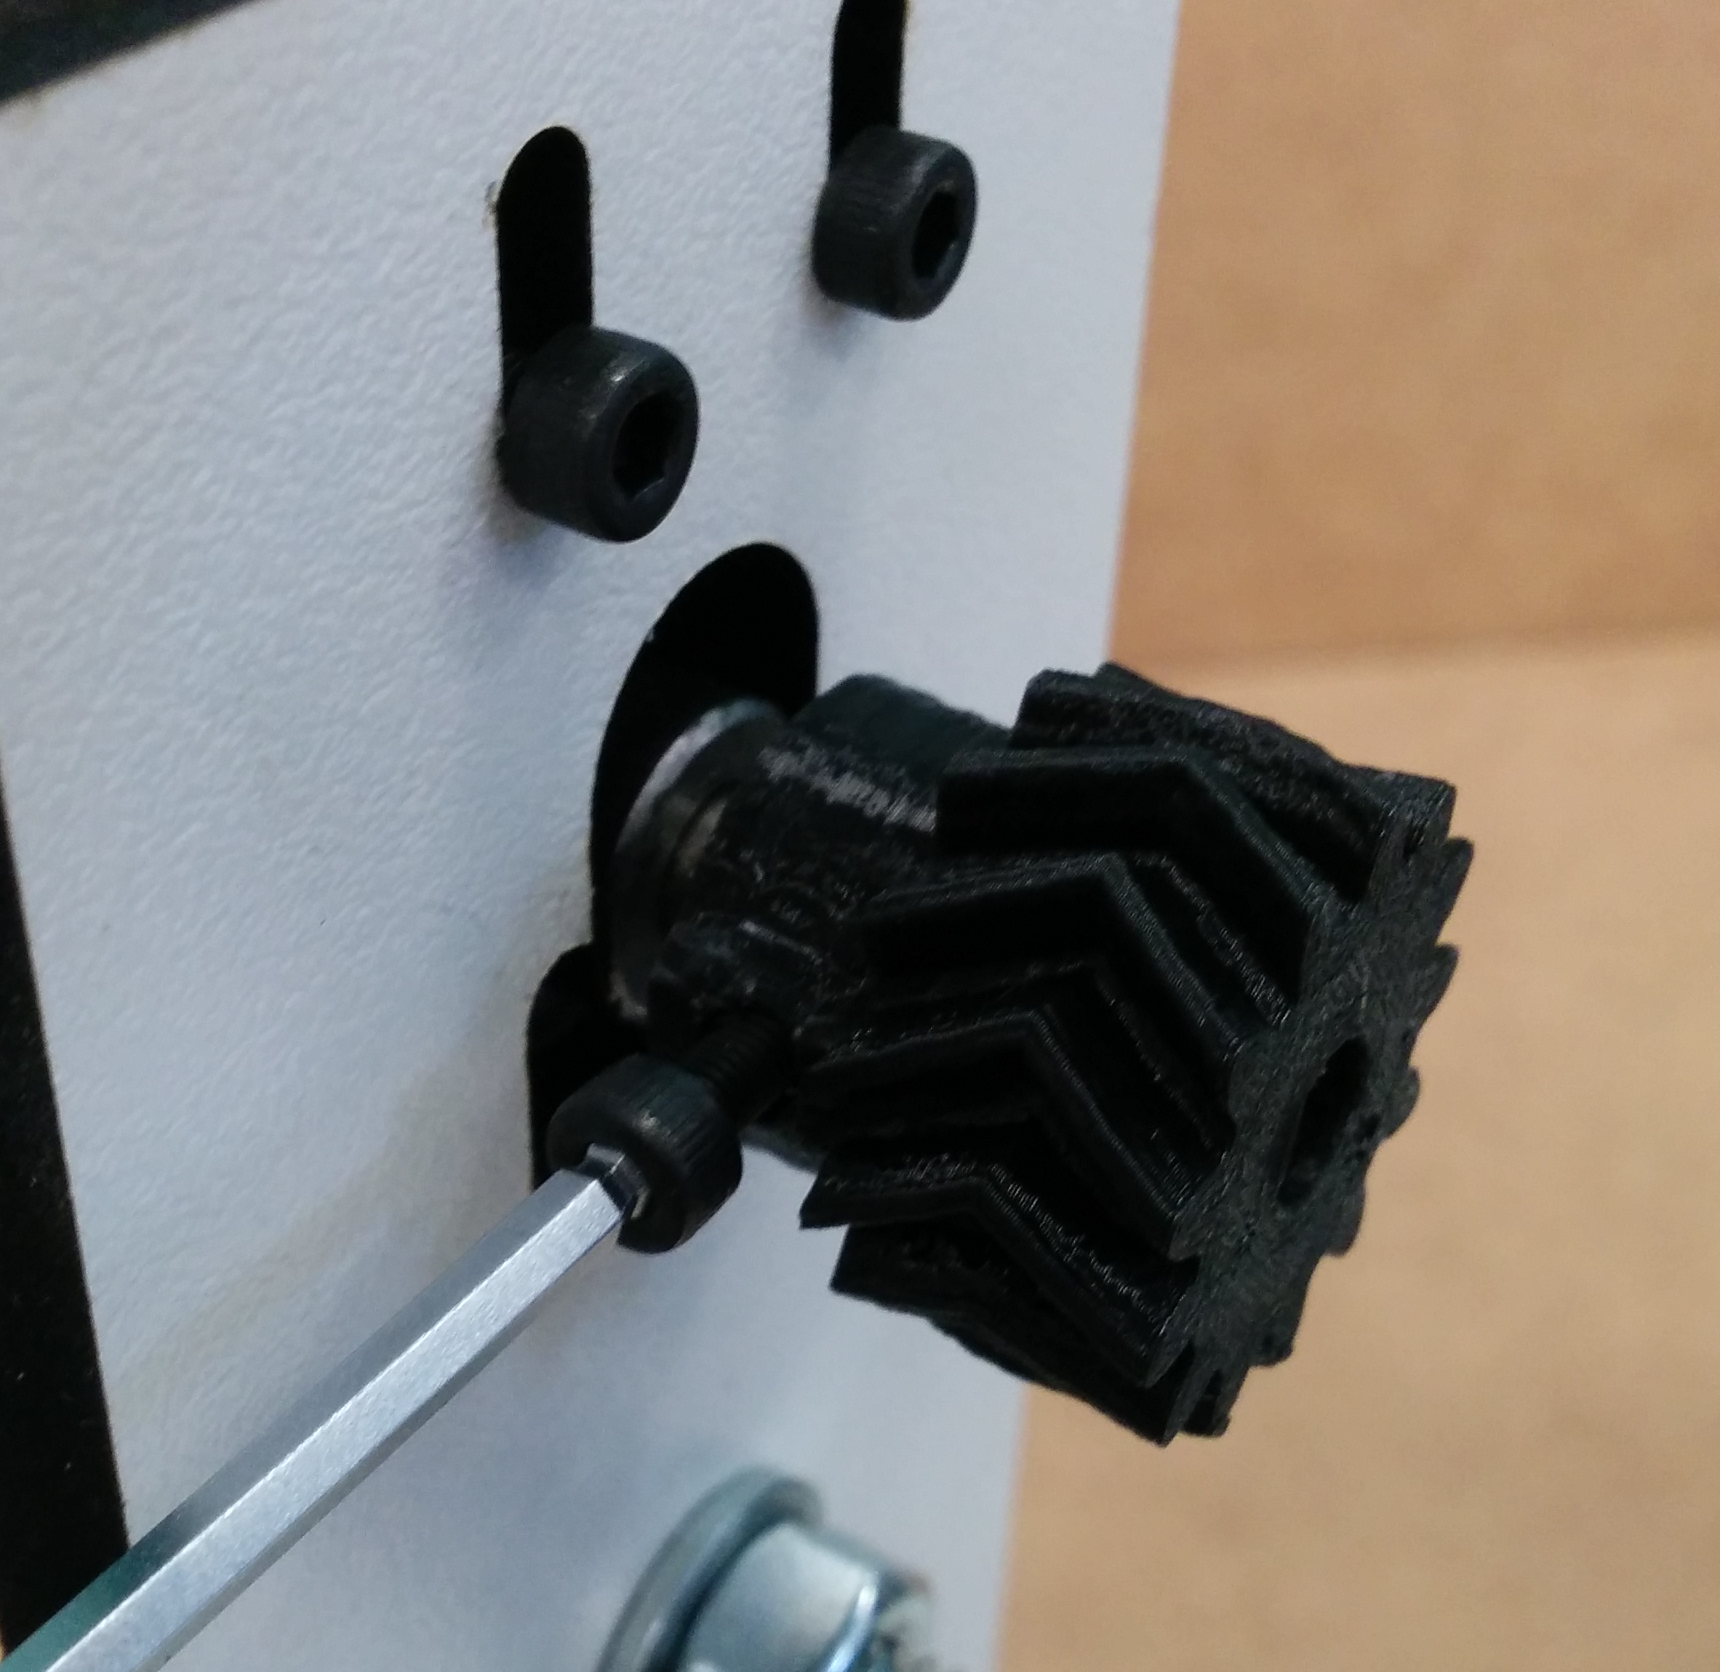
\includegraphics[width=\textwidth]{images/filawinder/montaje3.png}
                \caption{Apriete de engranaje al vástago.}
                \label{fig:winder_apriet}
        \end{subfigure}
        \caption{Montaje del engraneje en eje del motor.}
        \label{fig:winder_montaje_engranaje}
\end{figure}

Situamos la placa electrónica en la parte inferior de la pieza con ayuda de cuatro tornillos M3x12 y cuatro tuercas de M3.

    \begin{figure}[H]
            \centering
            \includegraphics[width=0.5\textwidth]{images/filawinder/montaje4.png}
            \caption{Instalación de la placa electrónica.}
            \label{fig:winder_arduino}
    \end{figure}

Roscamos una tuerca M8 e introducimos una arandela de M8 en la varilla roscada de M8, pasamos la varilla roscada a través del agujero debajo del motor, e introducimos otra arandela y otra tuerca de M8 para apretar el conjunto.

    \begin{figure}[H]
            \centering
            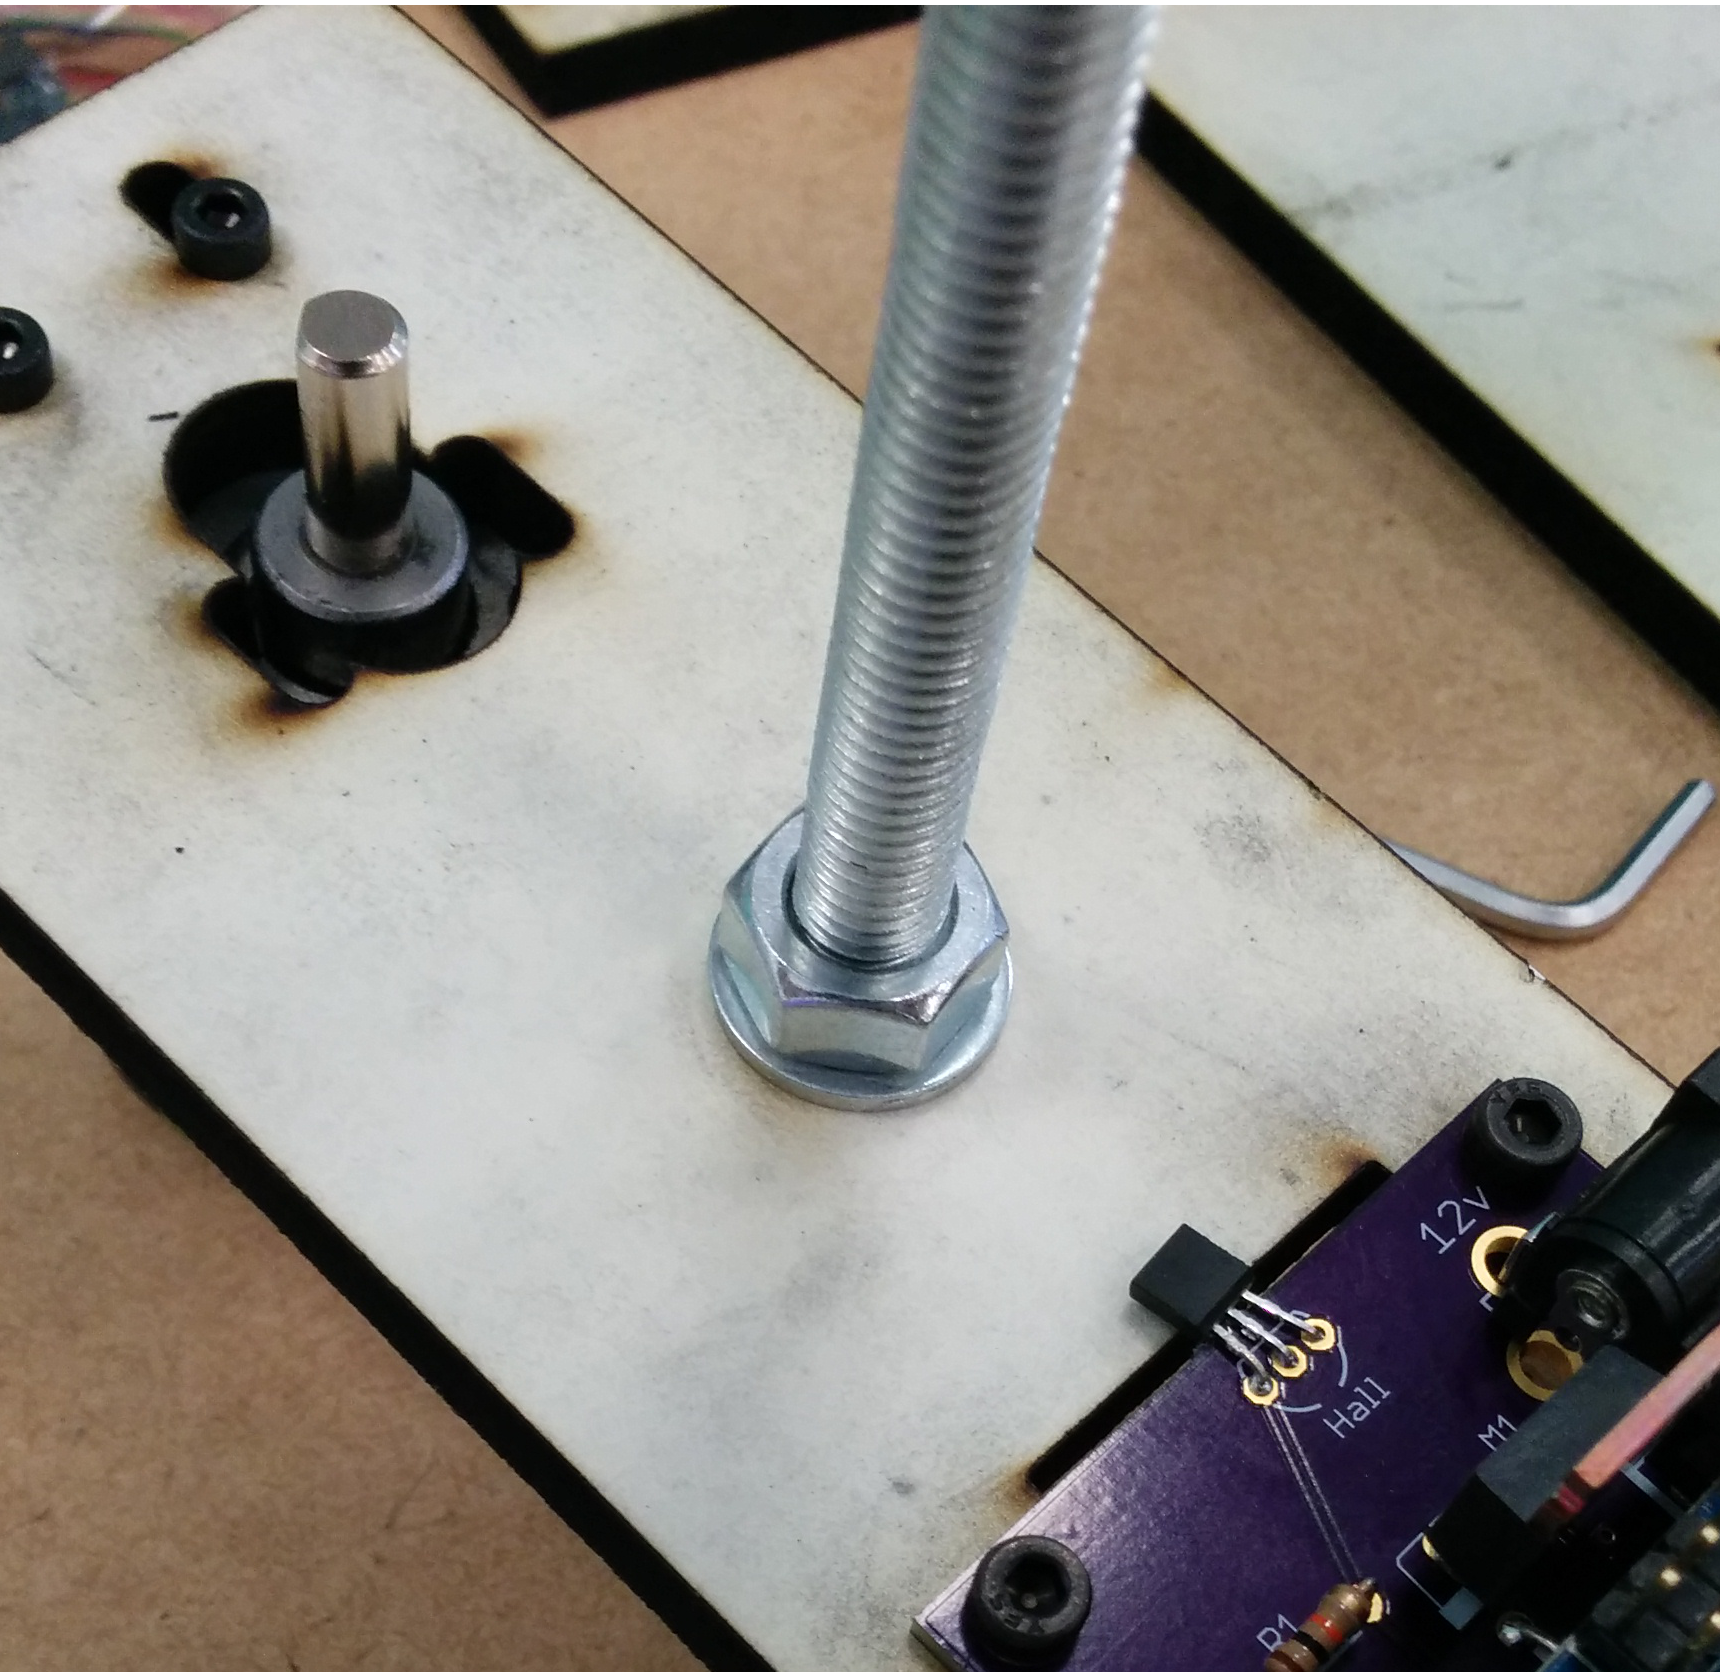
\includegraphics[width=0.5\textwidth]{images/filawinder/montaje5.png}
            \caption{Eje de giro para la bobina.}
            \label{fig:winder_soporte}
    \end{figure}

Alojamos la pieza con el motor, la varilla y la electrónica, en el lateral de la base principal, sujetamos ambas piezas con ayuda de una tuerca y un tornillo de M3x25.

    \begin{figure}[H]
            \centering
            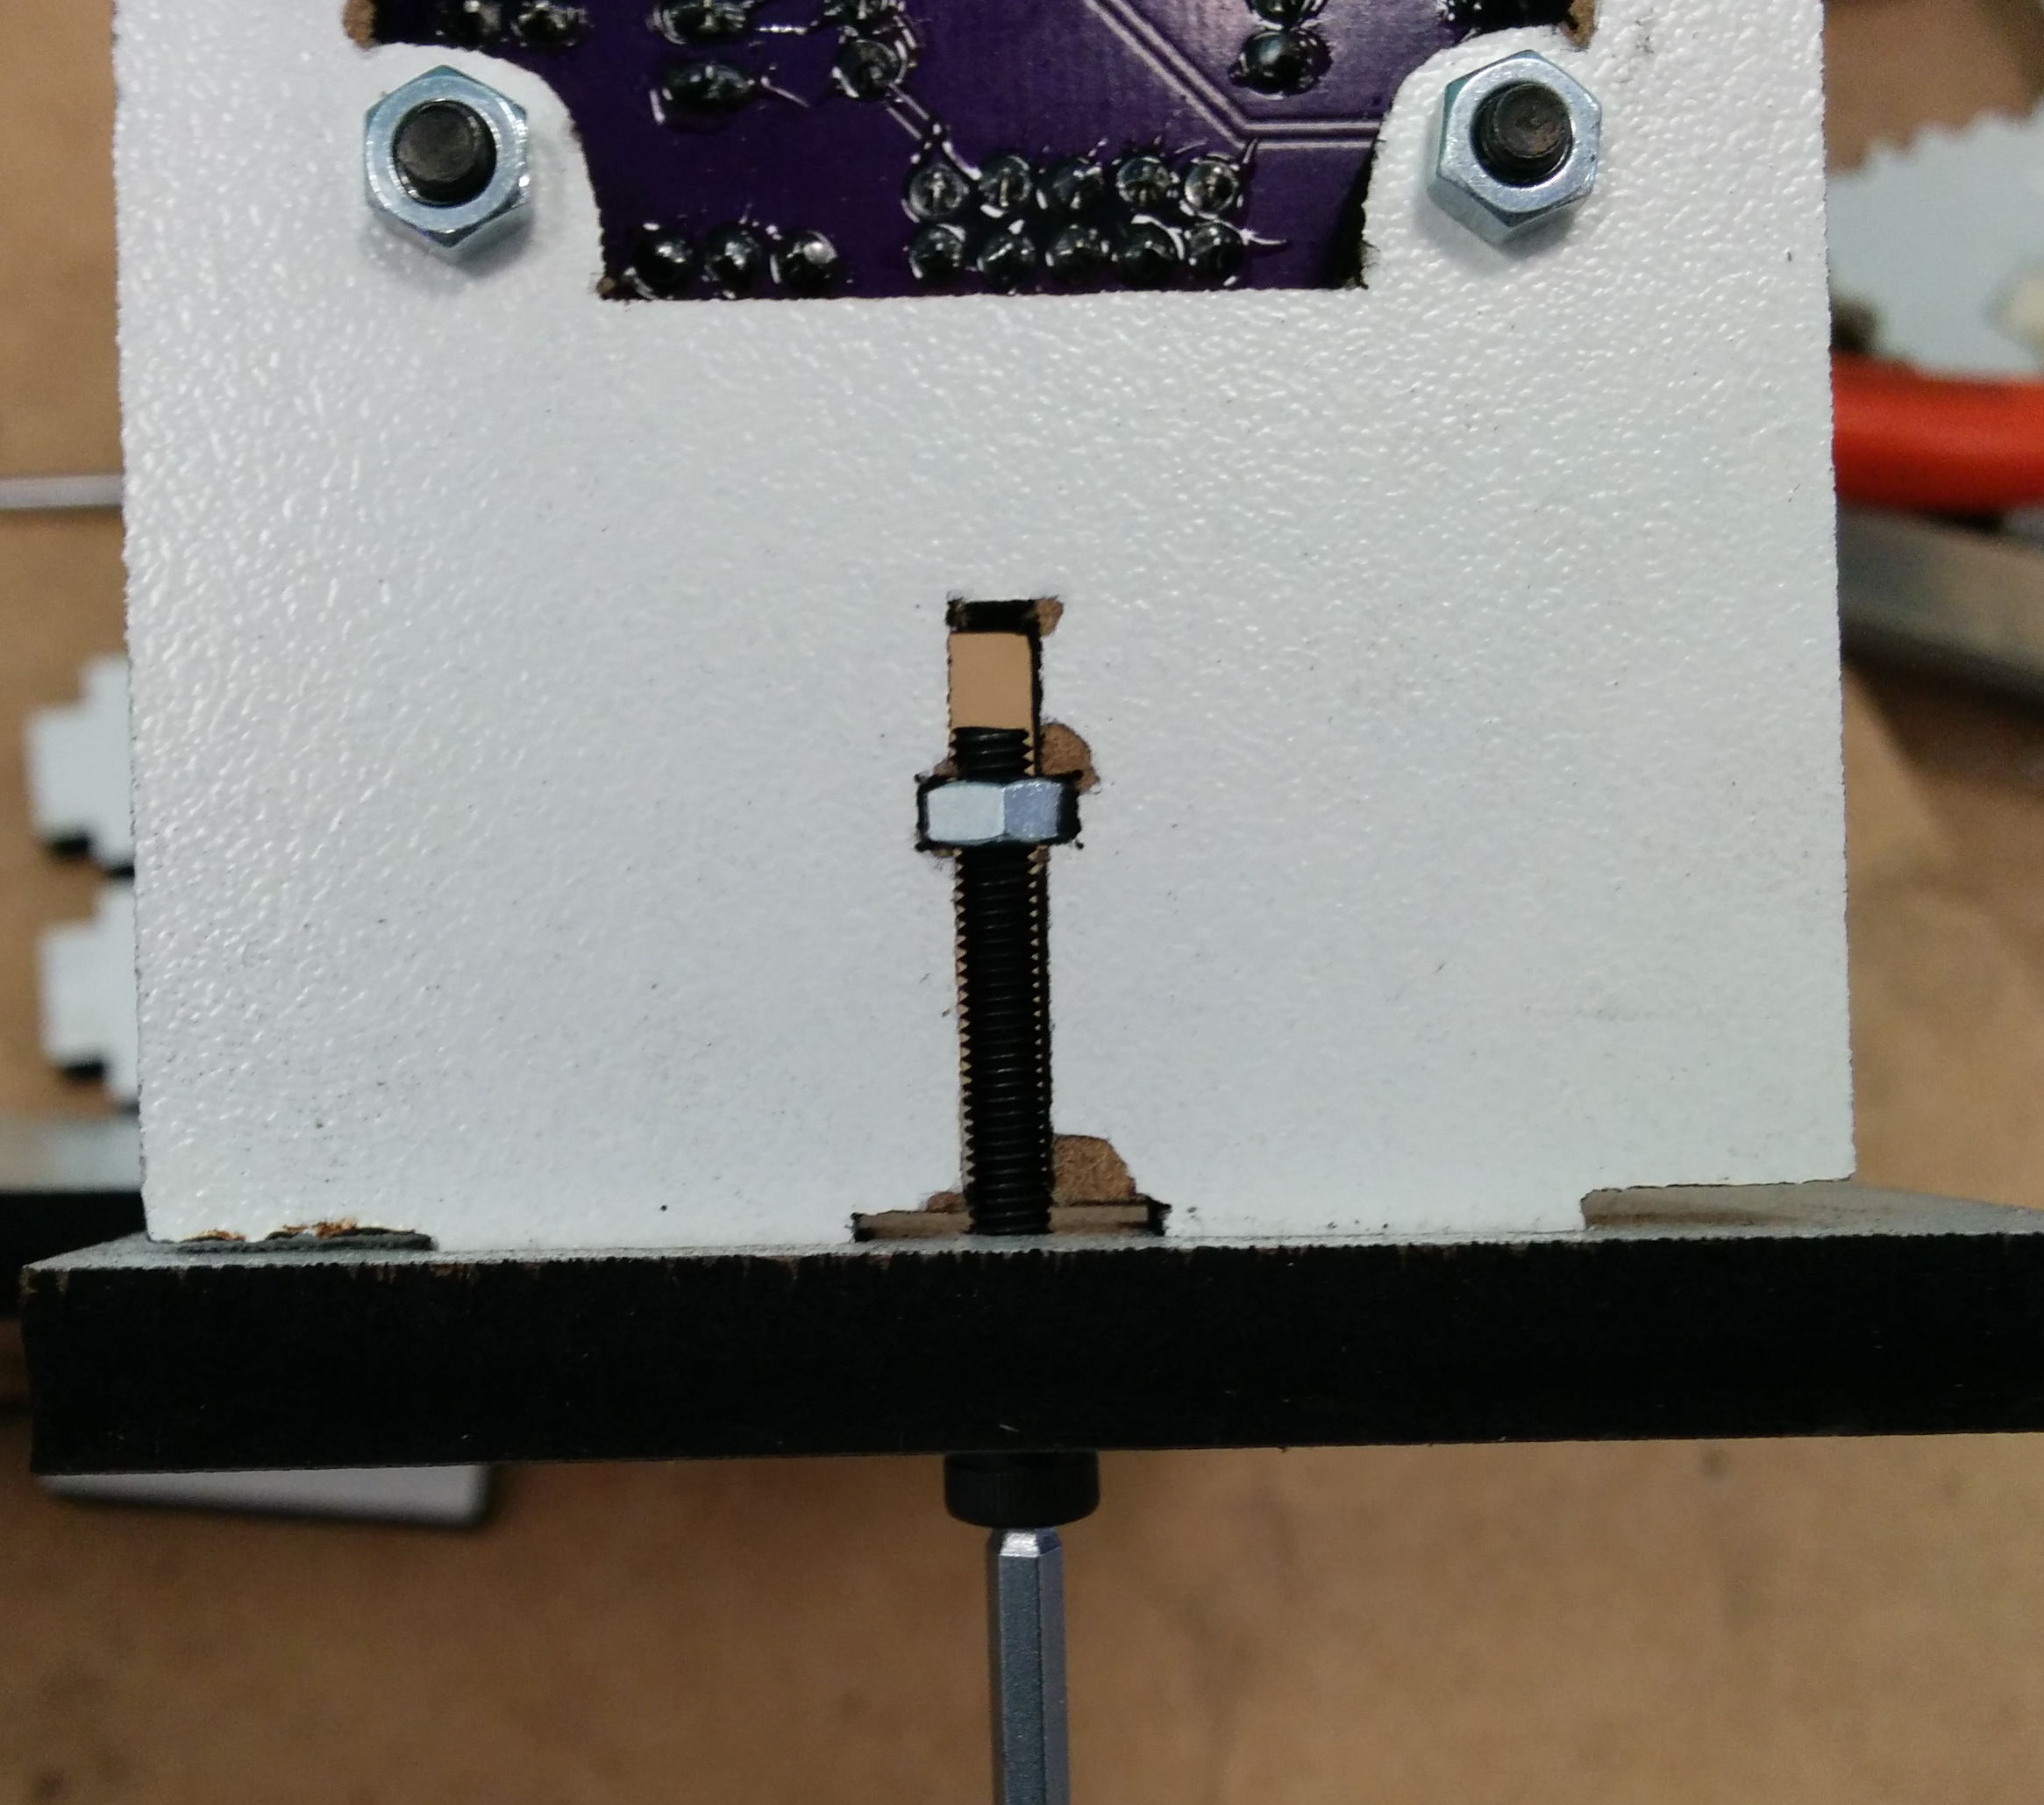
\includegraphics[width=0.5\textwidth]{images/filawinder/montaje6.png}
            \caption{Unión de lateral con base principal.}
            \label{fig:winder_soporte_base}
    \end{figure}


Una vez montada la estructura principal, sérá necesario cablear todos los componentes entre sí. 

    \begin{figure}[H]
          \centering
        \begin{subfigure}[b]{0.35\textwidth}
                \centering
                \includegraphics[width=\textwidth]{images/filawinder/IMG_20150311_123035.jpg}
                \caption{Botonera de control filawinder}
                \label{fig:winder_botonera}
        \end{subfigure}
        ~
        \begin{subfigure}[b]{0.35\textwidth}
                \centering
                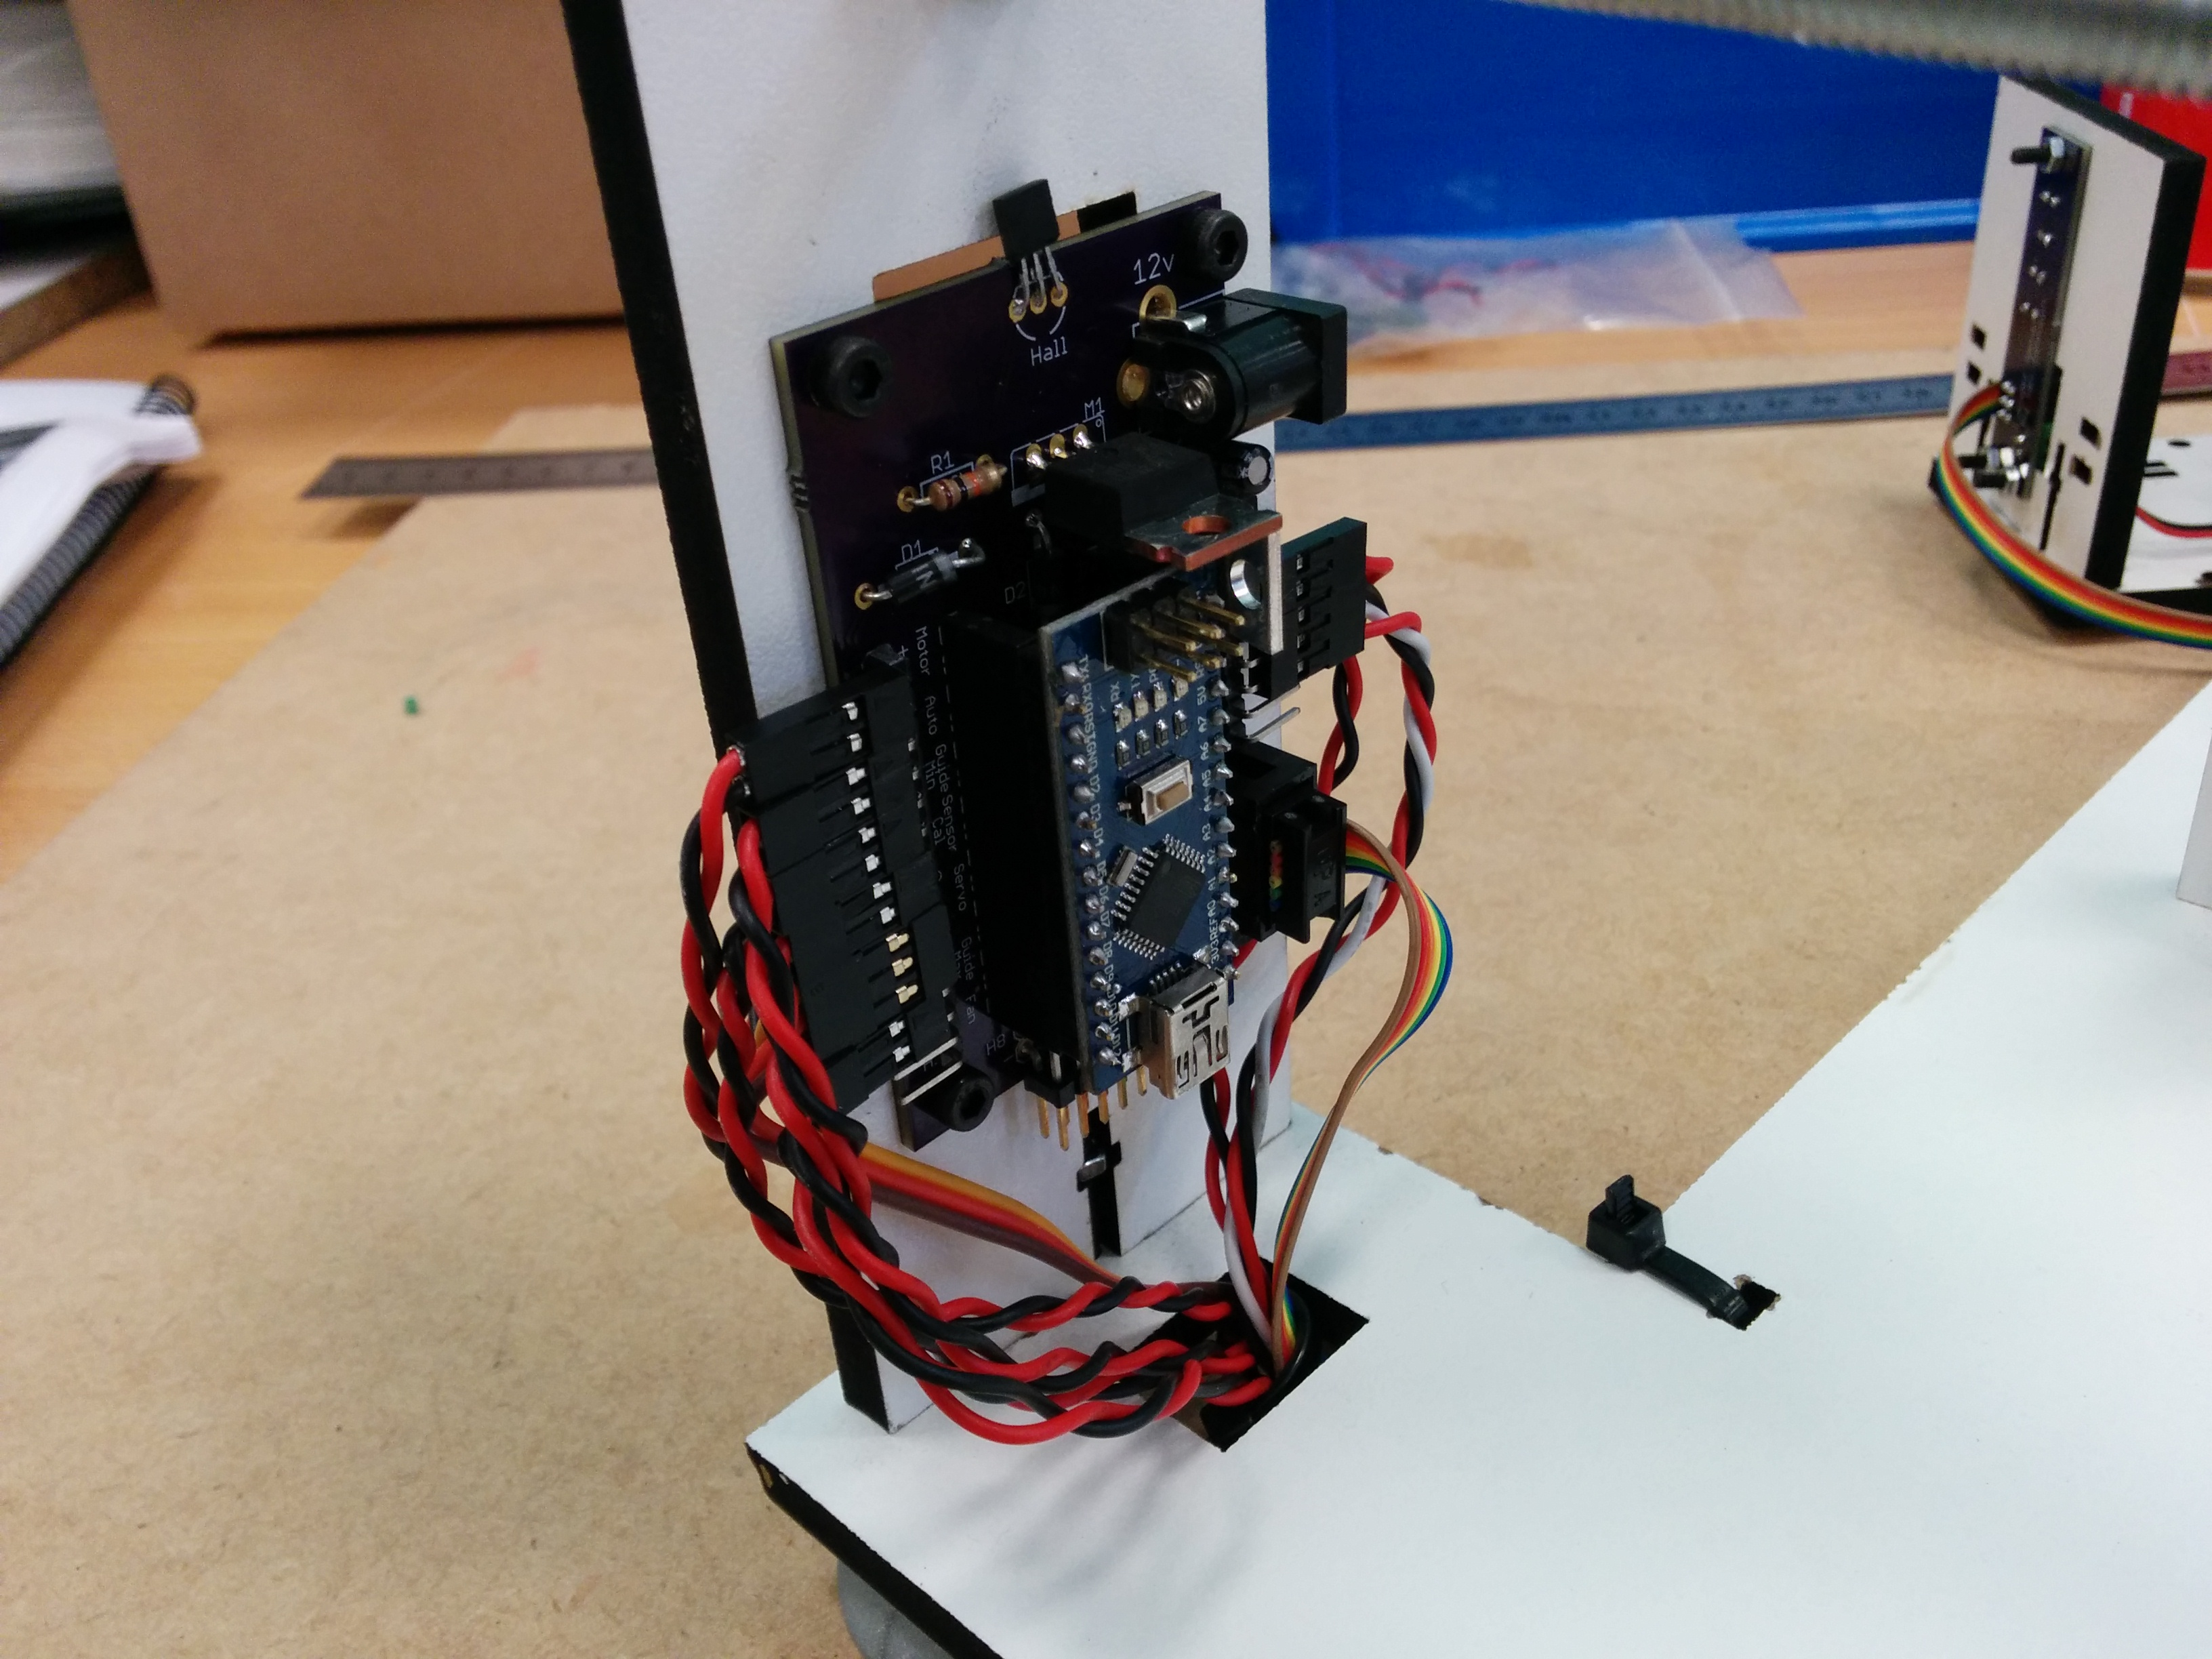
\includegraphics[width=\textwidth]{images/filawinder/IMG_20150311_131828.jpg}
                \caption{Placa controladra cableada.}
                \label{fig:winder_arduino1}
        \end{subfigure}
        \caption{Montaje electrico de la placa de control.}
        \label{fig:winder_montaje_electrio}
\end{figure}

Con esto concluimos el montaje del filawinder, el cual usaremos a la hora de producir filamento.
